\section{The Billing Framework architecture}\label{sec:the-code-derivation-pipeline}

As mentioned in section \addref rule-based systems require constant maintenance and rule updates.
Uncovered possible edge cases can appear even after system release.

As denoted in \addref one of the requirements for a rule-based system is extendability.
This does not only refer to the rules in the rule-base but also to the framework itself.
It must be straight forward to add new condition fields to the rule language.
This is why
I put great emphasis on extendability during the design of the Billing Framework
by making use of the pattern illustrated in figure \ref{fig:condition-triplet-pattern}.


\begin{figure}
    \centering
    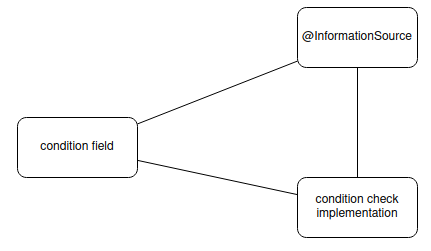
\includegraphics[width=0.75\linewidth]{./figures/condition-triplet-pattern}
    \caption{Geneic illustration of the triplet pattern}
    \label{fig:condition-triplet-pattern}
\end{figure}

Figure \addref and figure \addref display concrete instances of this pattern.


\begin{figure}
    \centering
    \begin{subfigure}[b]{0.45\linewidth}
        \centering
        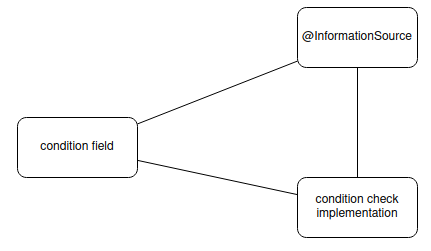
\includegraphics[width=\linewidth]{./figures/condition-triplet-pattern}
        \caption{Condition Triplet pattern instance 1}
        \label{fig:condition-triplet-pattern-instance-1}
    \end{subfigure}
    % Adjust or remove the space between figures as needed
    \hspace{5mm} % This adds a bit of horizontal space between the figures
    \begin{subfigure}[b]{0.45\linewidth}
        \centering
        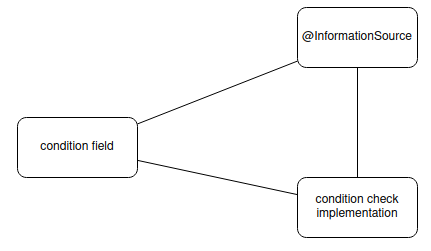
\includegraphics[width=\linewidth]{./figures/condition-triplet-pattern}
        \caption{Condition Triplet pattern instance 2}
        \label{fig:condition-triplet-pattern-instance-2}
    \end{subfigure}
    \label{fig:coffee}
\end{figure}



\subsection{Rule File Repository}


\subsection{Billing server}




\subsubsection{Rule Component}

\subsubsection{Rule Evaluation Input Fetcher}
A \code{RuleEvaluationInputFetcher} is a rule-type specific component responsible for fetching billing-relevant information from other services with the \AV microservice architecture.
They are auto-programmable components that hide fetching details from the rest of the system.
The term \"auto-programmable\" means that they configure themselves automatically upon rule loading.
This works as follows: The \code{Rule} entity class has as described before multiple condition fields.
The condition field names are equal to their corresponding condition keys in the rule language.
For each information source \todo{define information source}



It has access to the mi



